\chapter{Modelo de aprendizaje automático: diseño experimental y validación}\label{chapter-ml}

Este capítulo documenta el modelo supervisado que complementa al score descriptivo (RF07): qué se predice, con qué datos, cómo se separaron entrenamiento y validación, qué controles se aplicaron contra la fuga de información y qué resultados se obtuvieron. Reemplaza la evaluación del primer checkpoint del 22/09/2026, cuyas métricas resultaron optimistas por las razones que se explican en la Sección~\ref{sec:control-fuga}. Todas las cifras de este capítulo se generan con un único script versionado (\texttt{ml/train\_model.py}) y quedan registradas en \texttt{ml/model\_card.json}, de modo que cualquier valor citado puede rastrearse hasta su origen.

\section{Nomenclatura}\label{sec:nomenclatura}

Para evitar ambigüedades, en todo el documento se usan los siguientes términos con un único significado:

\begin{table}[H]
	\centering
	\small
	\caption{Nomenclatura del sistema. Fuente: elaboración propia.}
	\label{tab:nomenclatura}
	\begin{tabularx}{\textwidth}{@{}>{\raggedright\arraybackslash}p{2.6cm} X >{\raggedright\arraybackslash}p{3.6cm}@{}}
		\toprule
		\textbf{Término} & \textbf{Definición} & \textbf{Identificador} \\
		\midrule
		Producto & Referencia comercial del catálogo de Mercado Libre (por ejemplo, un modelo puntual de celular). Es la unidad de análisis: el score, la etiqueta y el índice ML se calculan por producto. & Fila de \texttt{Product}; clave \texttt{catalogProductId} cuando existe \\
		Publicación & Aviso puntual de un vendedor que ofrece un producto. Un producto puede tener varias publicaciones. & \texttt{mlId} (la más barata en la última corrida) \\
		Vendedor & Cuenta que ofrece una publicación. & \texttt{sellerId} \\
		Corrida & Ejecución de la minería (tres por día, Sección~\ref{sec:gestion-datasets}). & -- \\
		Aparición & Registro de que un producto apareció en los resultados de una corrida. & Fila de \texttt{TrendSnapshot} \\
		Score & Indicador descriptivo de 0 a 100 calculado sobre una ventana de 7 días (Ecuación~\ref{eq:score}). & Fila de \texttt{TrendScore} \\
		Etiqueta & Variable objetivo del modelo: 1 si el score sube al menos 5 puntos entre una corrida y la siguiente, 0 si no. & Columna \texttt{label} del dataset \\
		Tendencia & Concepto de negocio: crecimiento observable y sostenido de un producto en el tiempo (Sección~\ref{sec:concepto-central}). & -- \\
		Índice ML & Salida del modelo, expresada de 0 a 100. Ordena productos por prioridad; no es una probabilidad (Sección~\ref{sec:ml-calibracion}). & Campo \texttt{probability} de \texttt{MLPrediction} \\
		\bottomrule
	\end{tabularx}
\end{table}

Al corte del informe, 71 de los 310 productos registrados tienen \texttt{catalogProductId}. Los restantes se capturaron antes de que la identidad se resolviera contra el catálogo (Sección~\ref{sec:concepto-central}) y siguen identificados por la publicación con la que se registraron. El campo de la base que guarda el índice ML conserva el nombre técnico \texttt{probability} por compatibilidad con el esquema, pero su contenido se interpreta como índice.

\subsection*{Score, etiqueta y tendencia no son lo mismo}

La distinción es central para leer los resultados. El \textbf{score} describe el estado de un producto en una ventana de 7 días: cuánto aparece, hace cuánto, en qué posición, con qué estabilidad de precio y con cuánta competencia. La \textbf{etiqueta} mide un cambio de corto plazo de ese score: si sube al menos 5 puntos en la corrida siguiente (unas 8 horas después). La \textbf{tendencia}, en cambio, es lo que el vendedor quiere detectar: un crecimiento que se sostiene en el tiempo. La etiqueta es una aproximación operativa a la tendencia, no su definición: un salto de 5 puntos puede deberse a un crecimiento real, pero también a que un producto recién llegado está acumulando días dentro de su ventana (Sección~\ref{sec:variable-objetivo}). Por eso el índice ML se presenta como una señal de prioridad y no como una confirmación de tendencia.

\section{Versiones de datos y corte del informe}\label{sec:versiones-datos}

Las cifras del sistema crecen con cada corrida, y versiones anteriores de este documento mezclaban mediciones tomadas en fechas distintas (22/09, 23/09 y 24/09). Para eliminar esa inconsistencia, todas las cifras de volumen del informe se refieren a un único \textbf{corte de datos}: la corrida de minería del 09/10/2026 a las 07:19 (hora de Argentina). La Tabla~\ref{tab:versiones-datos} resume las versiones de datos y de modelo que se citan en el documento.

\begin{table}[H]
	\centering
	\small
	\caption{Versiones de datos y de modelo citadas en el informe. Fuente: elaboración propia, datos medidos en producción.}
	\label{tab:versiones-datos}
	\begin{tabularx}{\textwidth}{@{}>{\raggedright\arraybackslash}p{3cm} >{\raggedright\arraybackslash}p{2.6cm} X@{}}
		\toprule
		\textbf{Versión} & \textbf{Fecha} & \textbf{Contenido} \\
		\midrule
		Corte del informe & 09/10/2026, 07:19 & 86 días de captura (14/07 al 09/10/2026), $\sim$249 corridas (estimadas agrupando apariciones separadas por más de 40 minutos), 310 productos registrados (263 con score; 42 activos y 12 que dejaron de aparecer en los últimos 7 días), 6819 apariciones, 6909 registros de precio y 13.918 scores. Es la referencia de todas las cifras de volumen del documento. \\
		Dataset de ML & Exportado el 09/10/2026 & 13.655 pares de corridas consecutivas de 263 productos; 13.444 utilizables tras los filtros de la Sección~\ref{sec:variable-objetivo}. Congelado en \texttt{ml/data/dataset.json.gz}, SHA-256 \texttt{b73a1efc76ae\ldots} \\
		Modelo vigente & \texttt{rf\_2026-10-09\_b73a1efc} & Random Forest entrenado con las 13.444 filas utilizables, después de evaluarlo según este capítulo. Es el que genera el índice ML en la aplicación (Sección~\ref{sec:ml-trazabilidad}). \\
		Checkpoint anterior (reemplazado) & 22/09/2026 & 11.312 ejemplos de 227 productos, evaluado con un corte temporal sin purga ni embargo. Se conserva solo como antecedente: sus métricas (AUC-ROC 0,903, \emph{recall} 0,807) ya no se usan. \\
		\bottomrule
	\end{tabularx}
\end{table}

Las diferencias con versiones anteriores del documento se explican por la fecha de medición, no por errores de conteo: por ejemplo, 274 productos con apariciones al 23/09 y 310 productos registrados al 09/10. Los tiempos de respuesta de la API (Tabla~\ref{tab:evidencia}) conservan la fecha de su propia medición, indicada en cada fila, porque se midieron sobre versiones específicas del código.

\section{Variable objetivo y etiquetado}\label{sec:variable-objetivo}

Cada par de scores consecutivos de un mismo producto, calculados en las corridas $t$ y $t+1$, genera un ejemplo. Las features se toman de la corrida $t$ y la etiqueta vale 1 si $\text{score}_{t+1} - \text{score}_t \geq 5$. El etiquetado es automático y retrospectivo, y se aplicaron dos filtros para que la etiqueta mida cambios del mercado y no artefactos:

\begin{itemize}
	\item \textbf{Huecos de tiempo}: se descartan los 129 pares cuyas corridas están separadas por más de 24 horas. Corresponden a productos que dejaron de aparecer y volvieron días o semanas después (el hueco máximo fue de 52 días); comparar esos dos scores no describe un cambio de una corrida a la siguiente.
	\item \textbf{Cambios de metodología del score}: se descartan los 82 pares que cruzan alguno de los dos cambios de la fórmula (cálculo de la estabilidad sobre el promedio entre vendedores, el 23/09, e incorporación de la saturación con pesos nuevos, el 24 y 25/09; Sección~\ref{sec:score-formal}). Entre los 65 pares que cruzan el cambio de pesos, el 46\,\% quedaba etiquetado como positivo, contra el 6\,\% habitual: esa ``subida'' medía el cambio de fórmula, no el mercado. Cada score persiste los pesos con que fue calculado, lo que permite detectar estos pares de forma automática.
\end{itemize}

Quedan 13.444 ejemplos, con 6,26\,\% de positivos.

\subsection*{Justificación del umbral de 5 puntos}

El umbral se eligió por consistencia con la alerta de crecimiento ya implementada (HU02): la etiqueta que aprende el modelo y la alerta que recibe el cliente usan la misma definición de ``subida''. La distribución de los cambios de score entre corridas consecutivas respalda además que 5 puntos separa un movimiento relevante de la fluctuación habitual: la mediana del cambio es 0, el rango intercuartílico va de $-0{,}9$ a $+1{,}2$ puntos (2,1 puntos de amplitud) y $+5$ corresponde al percentil 93,7. Es decir, solo uno de cada dieciséis cambios supera el umbral, y lo hace por más de dos rangos intercuartílicos.

La Tabla~\ref{tab:sensibilidad-umbral} muestra cómo cambia el problema con otros umbrales, evaluando siempre con el mismo esquema de la Sección~\ref{sec:control-fuga}.

\begin{table}[H]
	\centering
	\small
	\caption{Sensibilidad del umbral de la etiqueta. Fuente: elaboración propia, \texttt{ml/model\_card.json}.}
	\label{tab:sensibilidad-umbral}
	\begin{tabular}{@{}lccc@{}}
		\toprule
		\textbf{Umbral} & \textbf{Prevalencia} & \textbf{ROC-AUC} & \textbf{PR-AUC} \\
		\midrule
		$+3$ puntos & 13,95\,\% & 0,780 & 0,360 \\
		$+5$ puntos (adoptado) & 6,26\,\% & 0,802 & 0,203 \\
		$+7$ puntos & 2,69\,\% & 0,967 & 0,448 \\
		$+10$ puntos & 2,54\,\% & 0,976 & 0,449 \\
		\bottomrule
	\end{tabular}
\end{table}

Los umbrales de $+7$ y $+10$ obtienen métricas mucho mejores, pero eso no es una ventaja. Casi todos los saltos de 7 puntos son también de 10 (la prevalencia apenas cambia), lo que indica saltos estructurales y muy predecibles, como la entrada de un producto nuevo a la ventana, más que variaciones del mercado. El umbral de $+3$ etiqueta como positivos cambios que están cerca del ruido habitual. El de $+5$ queda entre ambos extremos y mantiene la coherencia con la alerta.

\subsection*{Estabilidad de la etiqueta}

Se analizaron tres aspectos:

\begin{itemize}
	\item \textbf{Sostenimiento}: de los 817 saltos de al menos 5 puntos con tres corridas posteriores disponibles, 773 (94,6\,\%) seguían al menos 5 puntos por encima del score de partida tres corridas después (aproximadamente un día). La etiqueta no capta un ruido de una sola corrida.
	\item \textbf{Estabilidad en el tiempo}: excluyendo la primera semana, incompleta, la proporción semanal de positivos varió entre 2,1\,\% y 12,9\,\%. Fue más alta entre fines de julio y mediados de agosto, cuando entraban más productos nuevos al sistema (entre 22 y 37 por semana, contra 5 a 23 en las semanas siguientes). La etiqueta no es estacionaria, y eso explica parte de la variación de las métricas entre cortes (Sección~\ref{sec:ml-generalizacion}).
	\item \textbf{Efecto de llenado de ventana}: el 70,1\,\% de los positivos ocurre durante los primeros 7 días de vida de un producto en el sistema, cuando su permanencia y su frecuencia suben por construcción a medida que acumula días dentro de la ventana. En ese período la proporción de positivos es 10,6\,\%; después baja a 3,2\,\%. Si la evaluación se restringe a productos con más de 7 días en el sistema, el modelo mantiene un ROC-AUC de 0,796, pero su PR-AUC baja a 0,116 (frente a una prevalencia de 0,040). Sigue aportando información, pero bastante menos que sobre el conjunto completo.
\end{itemize}

El tercer punto es la principal limitación metodológica del modelo: la etiqueta actual mezcla dos fenómenos, la llegada de productos nuevos y el crecimiento de productos ya establecidos. Ambos son relevantes para el vendedor (un producto que recién empieza a aparecer es, por definición, un candidato temprano), pero no deben confundirse. Separarlos con una etiqueta de horizonte más largo es uno de los criterios de validación final (Sección~\ref{sec:ml-alcance}).

\section{Features, entrenamiento y reproducibilidad}\label{sec:ml-reproducibilidad}

El modelo usa ocho features, todas conocidas en el instante $t$: los cuatro componentes del score disponibles en todo el período (frecuencia, permanencia, ranking y estabilidad, Sección~\ref{sec:score-formal}) y su variación respecto de la corrida anterior. Respecto del checkpoint del 22/09 se quitaron tres variables:

\begin{itemize}
	\item La variación porcentual de precio, porque se calculaba como $1 - \text{estabilidad}$ y por lo tanto duplicaba información.
	\item La categoría del producto, que aportaba menos del 3\,\% de la importancia y podía llevar al modelo a memorizar la tasa base de cada categoría. El desempeño por categoría se analiza aparte (Sección~\ref{sec:ml-sesgos}).
	\item La saturación, que existe solo desde el 25/09 (15\,\% de las filas) y no permite entrenar ni validar con un corte temporal.
\end{itemize}

La Tabla~\ref{tab:ml-config} reúne todo lo necesario para reproducir el entrenamiento. Al reejecutar el pipeline sobre el mismo dataset se obtiene un archivo de modelo binariamente idéntico, y las métricas coinciden hasta la décima cifra decimal.

\begin{table}[H]
	\centering
	\small
	\caption{Configuración reproducible del modelo vigente. Fuente: \texttt{ml/model\_card.json}.}
	\label{tab:ml-config}
	\begin{tabularx}{\textwidth}{@{}>{\raggedright\arraybackslash}p{3.4cm} X@{}}
		\toprule
		\textbf{Elemento} & \textbf{Valor} \\
		\midrule
		Versión del modelo & \texttt{rf\_2026-10-09\_b73a1efc} (fecha de los datos y prefijo del hash del dataset) \\
		Dataset & \texttt{ml/data/dataset.json.gz}, SHA-256 \texttt{b73a1efc76ae39a2\ldots}; se regenera con \texttt{scripts/export\_ml\_training\_data.js} \\
		Algoritmo & Random Forest \parencite{PedregosaEtAl2011}; Regresión Logística como baseline lineal \\
		Hiperparámetros & 300 árboles, profundidad máxima 8, mínimo 5 ejemplos por hoja \\
		Balanceo de clases & \texttt{class\_weight="balanced"} (ponderación inversa a la frecuencia de cada clase, sin sobremuestreo) \\
		Semilla & 42 (modelo, permutaciones y particiones de productos no vistos) \\
		Separación & Corte en el cuantil 80\,\% del tiempo, con purga y embargo de 7 días (Sección~\ref{sec:control-fuga}) \\
		Software & Python 3.10.4, scikit-learn 1.7.2, pandas 2.3.3, numpy 2.1.3 (fijados en \texttt{ml/requirements.txt}) \\
		Artefactos & \texttt{ml/model.joblib} (modelo y cortes de nivel), \texttt{ml/model\_card.json} (todas las métricas), \texttt{ml/results.md} (reporte legible) \\
		Ejecución & \texttt{python ml/train\_model.py} \\
		\bottomrule
	\end{tabularx}
\end{table}

El modelo que se despliega se entrena con las 13.444 filas, con los mismos hiperparámetros, una vez reportada la evaluación sobre la partición de validación. Es la práctica habitual: evaluar con un corte y desplegar con todos los datos disponibles.

\section{Separación temporal y control de fuga}\label{sec:control-fuga}

Una partición aleatoria permitiría entrenar con datos posteriores a los que se validan. En este problema hay además un segundo riesgo, más sutil: las ventanas de 7 días de corridas consecutivas comparten casi todas sus apariciones, de modo que dos filas cercanas en el tiempo están fuertemente correlacionadas aunque una quede de cada lado del corte. Para controlar ambos efectos se aplicó un corte temporal con purga y embargo \parencite{LopezDePrado2018,BergmeirBenitez2012}:

\begin{enumerate}
	\item \textbf{Corte}: el cuantil 80\,\% de las fechas de las features, que cae el 19/09/2026 a las 05:22.
	\item \textbf{Purga}: el entrenamiento incluye solo filas cuya etiqueta ya se conocía antes del corte, es decir, cuya corrida $t+1$ es anterior al corte. Así ninguna etiqueta de entrenamiento usa información posterior. Las features de entrenamiento van del 18/07 al 18/09 y la última etiqueta usada es del 19/09 a las 05:22.
	\item \textbf{Embargo}: la validación empieza 7 días después del corte (26/09 a las 05:22), igual al largo de la ventana del score. Ninguna ventana de validación comparte apariciones con una ventana de entrenamiento.
	\item \textbf{Verificación automática}: el script interrumpe la ejecución si la última etiqueta de entrenamiento no es anterior a la primera feature de validación.
\end{enumerate}

Resultan 10.708 filas de entrenamiento (219 productos, 6,85\,\% de positivos) y 1784 de validación (83 productos, del 26/09 al 08/10, 4,26\,\% de positivos). Las 952 filas restantes quedan purgadas o dentro del embargo. En cuanto a la dependencia entre observaciones de un mismo producto, 744 de las 1784 filas de validación (42\,\%) corresponden a productos que también aparecen en entrenamiento, aunque en otro período y sin ventanas compartidas. El 58\,\% restante son productos que el modelo nunca vio. La generalización a productos no vistos se evalúa además de forma explícita en la Sección~\ref{sec:ml-generalizacion}.

La Tabla~\ref{tab:control-fuga} cuantifica cuánto cambia la evaluación según el esquema de separación.

\begin{table}[H]
	\centering
	\small
	\caption{Efecto del esquema de separación sobre la evaluación del Random Forest. Fuente: elaboración propia, \texttt{ml/model\_card.json}.}
	\label{tab:control-fuga}
	\begin{tabularx}{\textwidth}{@{}X ccc@{}}
		\toprule
		\textbf{Esquema} & \textbf{ROC-AUC} & \textbf{PR-AUC} & \textbf{Prevalencia} \\
		\midrule
		Partición aleatoria (con fuga) & 0,934 & 0,497 & 0,067 \\
		Corte temporal con purga, sin embargo & 0,855 & 0,222 & 0,040 \\
		Corte temporal con purga y embargo (adoptado) & 0,802 & 0,203 & 0,043 \\
		Etiquetas de entrenamiento permutadas (10 repeticiones) & 0,517 $\pm$ 0,075 & 0,057 $\pm$ 0,031 & 0,043 \\
		\bottomrule
	\end{tabularx}
\end{table}

La partición aleatoria duplica la PR-AUC: ese es el tamaño de la fuga que se evita. Las métricas del checkpoint anterior (AUC-ROC 0,903) se obtuvieron con un corte sin purga ni embargo y quedaron en una zona intermedia, por lo que eran optimistas. La prueba con etiquetas permutadas funciona como control negativo: si el pipeline filtrara información de la etiqueta por otra vía, el modelo seguiría acertando con etiquetas al azar. Su ROC-AUC promedio de 0,517 muestra que no lo hace.

\section{Resultados en validación}\label{sec:ml-resultados}

Con una clase positiva del 4,3\,\% en validación, la exactitud (\emph{accuracy}) no es informativa: un modelo que nunca predice ``sube'' acierta el 95,7\,\% de las veces. Por eso se reportan la PR-AUC, que se compara contra la prevalencia como línea de azar y es más informativa que la ROC-AUC con clases desbalanceadas \parencite{SaitoRehmsmeier2015}, la matriz de confusión, la tasa de falsos positivos (FPR) y el comportamiento por umbral.

\begin{table}[H]
	\centering
	\small
	\caption{Resultados en validación (1784 filas, prevalencia 0,043). Fuente: elaboración propia, \texttt{ml/model\_card.json}.}
	\label{tab:ml-resultados}
	\begin{tabularx}{\textwidth}{@{}>{\raggedright\arraybackslash}X cccccc@{}}
		\toprule
		\textbf{Modelo y umbral} & \textbf{ROC-AUC} & \textbf{PR-AUC} & \textbf{Precisión} & \textbf{Recall} & \textbf{FPR} & \textbf{Alertas} \\
		\midrule
		Regresión Logística, 0,50 & 0,772 & 0,184 & 0,073 & 0,658 & 0,372 & 38,5\,\% \\
		Random Forest, 0,50 & 0,802 & 0,203 & 0,105 & 0,513 & 0,195 & 20,9\,\% \\
		Random Forest, 0,374 (recall objetivo) & 0,802 & 0,203 & 0,111 & 0,711 & 0,254 & 27,4\,\% \\
		\bottomrule
	\end{tabularx}
\end{table}

\begin{figure}[htbp]
	\centering
	\begin{minipage}{0.56\textwidth}
		\centering
		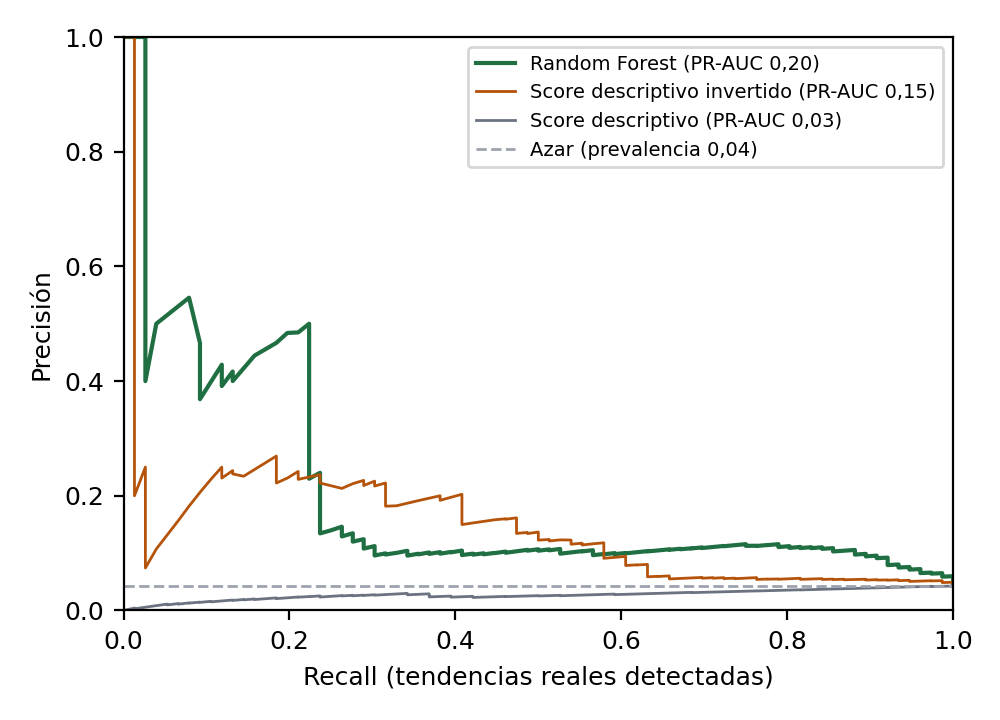
\includegraphics[width=\textwidth]{./images/ml/pr_curve.png}
	\end{minipage}\hfill
	\begin{minipage}{0.40\textwidth}
		\centering
		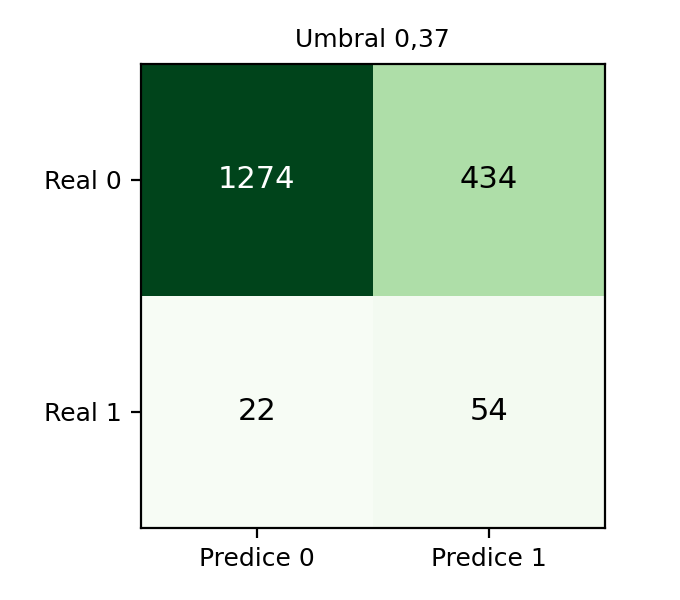
\includegraphics[width=\textwidth]{./images/ml/confusion_matrix.png}
	\end{minipage}
	\caption{Izquierda: curva precisión-recall del Random Forest frente al score descriptivo y al azar. Derecha: matriz de confusión al umbral que alcanza el recall objetivo. Validación del 26/09 al 08/10/2026. Fuente: elaboración propia.}
	\label{fig:ml-pr-confusion}
\end{figure}

El objetivo específico 5 fijaba un \emph{recall} mínimo de 0,70 para la clase positiva. El Random Forest lo alcanza con un umbral de 0,374: detecta 54 de las 76 subidas reales de validación (\emph{recall} 0,711), pero lo hace con 434 falsos positivos. Su precisión es de 0,111, es decir, se confirma una de cada nueve señales, y marca el 27,4\,\% de los casos. Frente a la línea de azar, la PR-AUC de 0,203 es 4,8 veces la prevalencia. La Tabla~\ref{tab:ml-umbrales} muestra el compromiso completo entre recall y falsas alertas.

\begin{table}[H]
	\centering
	\small
	\caption{Comportamiento del Random Forest por umbral (validación). Fuente: elaboración propia, \texttt{ml/model\_card.json}.}
	\label{tab:ml-umbrales}
	\begin{tabular}{@{}ccccc@{}}
		\toprule
		\textbf{Umbral} & \textbf{Precisión} & \textbf{Recall} & \textbf{FPR} & \textbf{Casos marcados} \\
		\midrule
		0,20 & 0,070 & 0,961 & 0,567 & 58,4\,\% \\
		0,30 & 0,098 & 0,882 & 0,361 & 38,3\,\% \\
		0,40 & 0,099 & 0,592 & 0,241 & 25,6\,\% \\
		0,50 & 0,105 & 0,513 & 0,195 & 20,9\,\% \\
		0,70 & 0,102 & 0,461 & 0,181 & 19,3\,\% \\
		0,90 & 0,391 & 0,118 & 0,008 & 1,3\,\% \\
		\bottomrule
	\end{tabular}
\end{table}

La lectura es clara: el modelo ordena bien los productos según su chance de subir, pero no alcanza la precisión necesaria para disparar alertas automáticas sin revisión. Solo en la franja más alta (umbral 0,90) la precisión llega a 0,39, a cambio de detectar apenas el 12\,\% de las subidas. Por eso se usa como criterio de priorización dentro del tablero y no como disparador de alertas (Sección~\ref{sec:ml-trazabilidad}).

\section{Comparación contra reglas simples y el score descriptivo}\label{sec:ml-baselines}

Un modelo solo se justifica si supera alternativas más simples. Se compararon cuatro, evaluadas sobre la misma partición de validación:

\begin{table}[H]
	\centering
	\small
	\caption{Random Forest frente a reglas simples y al score descriptivo (validación). Fuente: elaboración propia, \texttt{ml/model\_card.json}.}
	\label{tab:ml-baselines}
	\begin{tabularx}{\textwidth}{@{}X cccc@{}}
		\toprule
		\textbf{Método} & \textbf{ROC-AUC} & \textbf{PR-AUC} & \textbf{Precisión} & \textbf{Recall} \\
		\midrule
		Azar (prevalencia) & 0,500 & 0,043 & -- & -- \\
		Regla: la frecuencia de aparición aumentó & 0,553 & 0,048 & 0,052 & 0,579 \\
		Regla: el score ya subió 5 puntos en la corrida anterior & 0,521 & 0,046 & 0,076 & 0,092 \\
		Score descriptivo (más alto, más chance) & 0,287 & 0,028 & -- & -- \\
		Score descriptivo invertido (más bajo, más chance) & 0,713 & 0,147 & -- & -- \\
		Random Forest & \textbf{0,802} & \textbf{0,203} & 0,105 & 0,513 \\
		\bottomrule
	\end{tabularx}
\end{table}

Las dos reglas intuitivas quedan prácticamente en el nivel del azar: que la frecuencia esté aumentando o que el producto ya haya subido no anticipa la próxima subida. El score descriptivo muestra una relación \emph{inversa} con la etiqueta (ROC-AUC 0,287): los productos con score alto casi no tienen margen para subir 5 puntos más. Su versión invertida es la alternativa más competitiva (PR-AUC 0,147), porque captura justamente que los productos con score bajo son los que pueden subir. El Random Forest la supera en un 38\,\% en PR-AUC y en 0,09 de ROC-AUC, lo que justifica su uso como complemento del score. Este resultado aclara además el rol de cada herramienta: el score describe qué productos ya están en tendencia y el índice ML prioriza entre los que todavía no lo están.

\section{Generalización: origen móvil y productos no vistos}\label{sec:ml-generalizacion}

Un único corte puede dar una imagen favorable o desfavorable por azar. Para medir la estabilidad se repitió la evaluación con origen móvil: tres cortes sucesivos, cada uno con purga y embargo de 7 días.

\begin{table}[H]
	\centering
	\small
	\caption{Evaluación con origen móvil. Fuente: elaboración propia, \texttt{ml/model\_card.json}.}
	\label{tab:ml-origen-movil}
	\begin{tabular}{@{}lccccc@{}}
		\toprule
		\textbf{Corte} & \textbf{Filas de validación} & \textbf{Prevalencia} & \textbf{ROC-AUC} & \textbf{PR-AUC} & \textbf{Recall (0,50)} \\
		\midrule
		03/09/2026 & 4059 & 0,039 & 0,861 & 0,280 & 0,633 \\
		11/09/2026 & 2868 & 0,038 & 0,874 & 0,278 & 0,618 \\
		19/09/2026 (adoptado) & 1784 & 0,043 & 0,802 & 0,203 & 0,513 \\
		\bottomrule
	\end{tabular}
\end{table}

Las métricas se mantienen siempre muy por encima del azar, pero bajan en el corte más reciente. La causa más probable es que la validación de ese corte cae íntegramente después de los dos cambios de metodología del score (23 al 25/09), mientras que el entrenamiento usa la fórmula anterior. Se reporta el corte más reciente, que es el menos favorable, porque es el que mejor representa el funcionamiento actual del sistema.

Para evaluar la \textbf{generalización a productos no vistos} se repitió cinco veces el siguiente procedimiento: se aparta al azar el 20\,\% de los productos, se entrena sin ninguna fila de ellos y se valida solo sobre ellos, después del embargo. En las cinco repeticiones (entre 13 y 17 productos y entre 279 y 342 filas cada una) el ROC-AUC promedio fue de 0,848 (desvío 0,063) y la PR-AUC promedio de 0,311 (desvío 0,164), frente a una prevalencia promedio de 0,037. El desempeño sobre productos nuevos no es inferior al general. Esto es esperable por el diseño de las features: el modelo no recibe identificadores de producto ni de categoría, sino componentes normalizados del score, que significan lo mismo para cualquier producto. Lo que aprende es la dinámica de esos componentes y no la identidad de los productos. El desvío alto entre repeticiones refleja que cada una evalúa pocos productos, por lo que el promedio debe leerse como orientativo.

\section{Desempeño por categoría, cobertura y sesgos}\label{sec:ml-sesgos}

\begin{table}[H]
	\centering
	\small
	\caption{Cobertura del dataset y desempeño en validación por categoría (umbral 0,50). Fuente: elaboración propia, \texttt{ml/model\_card.json}.}
	\label{tab:ml-categorias}
	\begin{tabularx}{\textwidth}{@{}>{\raggedright\arraybackslash}X ccccccc@{}}
		\toprule
		 & \multicolumn{2}{c}{\textbf{Dataset}} & \multicolumn{5}{c}{\textbf{Validación}} \\
		\cmidrule(lr){2-3}\cmidrule(l){4-8}
		\textbf{Categoría} & \textbf{Filas} & \textbf{Prod.} & \textbf{Positivos} & \textbf{ROC-AUC} & \textbf{PR-AUC} & \textbf{Recall} & \textbf{FPR} \\
		\midrule
		Limpieza del Hogar & 5004 & 93 & 26 & 0,777 & 0,215 & 0,538 & 0,280 \\
		Computación & 2187 & 35 & 13 & 0,778 & 0,062 & 0,308 & 0,139 \\
		Electrónica & 1995 & 49 & 7 & 0,849 & 0,527 & 0,571 & 0,193 \\
		Celulares & 1965 & 47 & 22 & 0,833 & 0,436 & 0,636 & 0,233 \\
		Alimentos y Bebidas & 1788 & 32 & 8 & 0,686 & 0,063 & 0,375 & 0,162 \\
		Ropa y Accesorios & 505 & 7 & 0 & -- & -- & -- & 0,105 \\
		\bottomrule
	\end{tabularx}
\end{table}

El análisis por categoría muestra sesgos que limitan el alcance de los resultados:

\begin{itemize}
	\item \textbf{Cobertura desigual}: Limpieza del Hogar aporta el 37\,\% de las filas, mientras que Ropa y Accesorios tiene solo 7 productos y ningún positivo en validación, por lo que su desempeño no puede evaluarse.
	\item \textbf{Desempeño desigual}: en Celulares y Electrónica la PR-AUC multiplica varias veces la prevalencia, pero en Computación y en Alimentos y Bebidas queda cerca del azar. En esas categorías el índice ML no debería usarse todavía como criterio de priorización. Además, las categorías con pocos positivos (7 u 8) tienen métricas muy inestables.
	\item \textbf{Sesgo de selección}: el sistema observa solo los productos que aparecen en las búsquedas de la minería (8 por categoría y palabra clave), no el catálogo completo. Los resultados describen a esa población y no son extrapolables a cualquier producto de Mercado Libre.
	\item \textbf{Sesgo hacia productos nuevos}: el 70\,\% de los positivos corresponde a productos en sus primeros 7 días (Sección~\ref{sec:variable-objetivo}).
	\item \textbf{Cambios de identidad y de metodología}: hasta el 23/09, un cambio del vendedor más barato podía cortar el histórico de un producto, y los datos de cantidad de vendedores existen solo desde esa fecha. Ambos efectos afectan más a las primeras semanas del dataset.
\end{itemize}

\section{Calibración y denominación de la salida}\label{sec:ml-calibracion}

Para llamar ``probabilidad'' a la salida del modelo, un valor de 0,30 debería corresponder a productos que suben aproximadamente en el 30\,\% de los casos. Se verificó con el puntaje de Brier \parencite{Brier1950}, que mide el error cuadrático medio de las probabilidades (menor es mejor), y con la curva de calibración.

\begin{figure}[H]
	\centering
	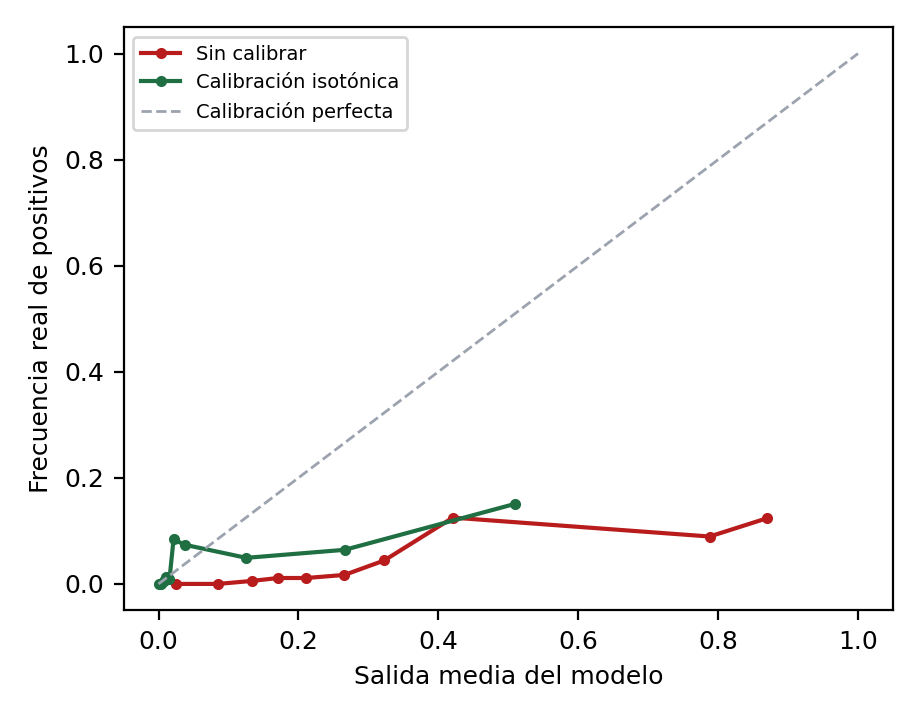
\includegraphics[width=0.55\textwidth]{./images/ml/calibration.png}
	\caption{Curva de calibración del Random Forest en validación, sin calibrar y con calibración isotónica. Fuente: elaboración propia.}
	\label{fig:ml-calibracion}
\end{figure}

Sin calibrar, la salida media del modelo es 0,329, cuando la frecuencia real de subidas es 0,043: el modelo sobreestima sistemáticamente. Es una consecuencia conocida del balanceo de clases \parencite{NiculescuMizilCaruana2005}. Su Brier es de 0,176, peor que el de una referencia trivial que asigna a todos los productos la prevalencia de entrenamiento (0,041), y su error de calibración esperado (ECE) es de 0,287. Se probó una calibración isotónica ajustada con tres particiones temporales dentro del entrenamiento. Mejora mucho (Brier 0,055, ECE 0,076), pero sigue sin superar a la referencia trivial y reduce levemente la PR-AUC (0,199).

Como la calibración no se verifica, la salida \textbf{no se presenta como probabilidad}. En la aplicación se muestra como \textbf{índice ML de 0 a 100}, aclarando que es una prioridad relativa, con tres niveles definidos sobre la validación:

\begin{itemize}
	\item \textbf{Alto} (37 o más): umbral que alcanza el recall objetivo de 0,70.
	\item \textbf{Medio} (de 20 a 37): umbral con recall de 0,96.
	\item \textbf{Bajo} (menos de 20).
\end{itemize}

Los cortes se guardan con el modelo, y un test automatizado verifica que la aplicación use exactamente los mismos valores que \texttt{ml/model\_card.json}. La columna que antes se llamaba ``Prob. ML'' en el ranking pasó a llamarse ``Índice ML''. Las capturas del Capítulo~\ref{chapter07} tomadas antes de este cambio muestran todavía el nombre anterior.

\section{Trazabilidad de la predicción}\label{sec:ml-trazabilidad}

La Tabla~\ref{tab:ml-trazabilidad} recorre el camino completo de una predicción, desde los datos de entrenamiento hasta lo que ve el cliente.

\begin{table}[H]
	\centering
	\small
	\caption{Trazabilidad del índice ML. Fuente: elaboración propia.}
	\label{tab:ml-trazabilidad}
	\begin{tabularx}{\textwidth}{@{}>{\raggedright\arraybackslash}p{2.3cm} >{\raggedright\arraybackslash}p{5.4cm} X@{}}
		\toprule
		\textbf{Etapa} & \textbf{Artefacto} & \textbf{Qué garantiza la trazabilidad} \\
		\midrule
		1. Dataset & \path{scripts/export_ml_training_data.js} $\rightarrow$ \path{ml/data/dataset.json.gz} & Hash SHA-256 registrado en la versión del modelo y en la \emph{model card}. \\
		2. Entrenamiento & \path{ml/train_model.py} $\rightarrow$ \path{ml/model.joblib}, \path{ml/model_card.json} & El modelo se guarda junto con su versión, sus features y los cortes de nivel. \\
		3. Ejecución periódica & \path{.github/workflows/mineria.yml}: minería, score, \path{export_latest_features.js}, \path{predict.py}, \path{import_ml_predictions.js} & Tres veces por día. Solo se predicen productos con score en las últimas 24 horas y con un score previo a menos de 24 horas, las mismas condiciones que en el entrenamiento. \\
		4. Persistencia & Tabla \texttt{MLPrediction} & Cada fila guarda producto, índice, fecha y \texttt{modelVersion}. \\
		5. API & \texttt{/api/trend-scores} y \texttt{/api/insights} & Solo devuelven predicciones de la versión vigente del modelo, para no mezclar valores de un modelo anterior. \\
		6. Visualización & Columna ``Índice ML'' del ranking; detalle de producto y pie del tablero de oportunidades & El tablero muestra la versión del modelo que generó los valores. \\
		7. Alertas & \path{scripts/generate_alerts.js} & Las alertas \textbf{no} usan el índice ML: se disparan con la regla del score (subida de al menos 5 puntos, HU02), la misma definición que la etiqueta. Es una decisión deliberada, dada la precisión de 0,11 del modelo (Sección~\ref{sec:ml-resultados}). \\
		\bottomrule
	\end{tabularx}
\end{table}

\section{Alcance de las conclusiones: de checkpoint a modelo validado}\label{sec:ml-alcance}

Con la evidencia de este capítulo puede afirmarse que el modelo:

\begin{itemize}
	\item ordena productos según su chance de subir en la corrida siguiente con información genuina: su PR-AUC es 4,8 veces la prevalencia, supera a todas las reglas simples y al score descriptivo invertido, y resiste los controles de fuga (purga, embargo y etiquetas permutadas);
	\item generaliza a productos que no vio durante el entrenamiento, con desempeño comparable al general;
	\item es reproducible: dataset congelado con hash, semilla fija y una versión rastreable hasta la aplicación.
\end{itemize}

No puede afirmarse, en cambio, que el sistema \emph{detecte tendencias de manera confiable}:

\begin{itemize}
	\item su precisión es baja (una de cada nueve señales se confirma con el recall objetivo) y su salida no está calibrada;
	\item la etiqueta mide una subida de corto plazo y está influida por la llegada de productos nuevos, por lo que no equivale a una tendencia sostenida;
	\item el histórico cubre 86 días y dos cambios de metodología del score, menos que un ciclo estacional completo, y la prevalencia de la etiqueta varía en el tiempo;
	\item en dos de las seis categorías el desempeño es cercano al azar y en una no es evaluable.
\end{itemize}

Por lo tanto, el estado del modelo es de \textbf{validación inicial}: es útil como señal de priorización dentro del tablero, con sus limitaciones explícitas, y no como detector autónomo. Para considerarlo validado se fijan los siguientes criterios, que se retoman en el trabajo futuro (Sección~\ref{sec:trabajo-futuro}):

\begin{enumerate}
	\item Al menos seis meses de histórico bajo la metodología actual del score, sin cambios de fórmula dentro del período evaluado.
	\item Una evaluación fuera de muestra de al menos dos meses con el modelo congelado, sin reentrenarlo durante ese período.
	\item Una etiqueta de horizonte más largo (por ejemplo, una subida sostenida durante tres días) que excluya el efecto de llenado de ventana de los productos nuevos.
	\item Una PR-AUC estable entre cortes del origen móvil, con un desvío menor al 20\,\% de su media.
	\item Una calibración que supere al puntaje de Brier de referencia, condición necesaria para volver a hablar de probabilidad.
	\item Al menos 30 positivos de validación por categoría antes de reportar o usar el índice en esa categoría.
\end{enumerate}
